%\documentclass[12pt,a4paper]{article}
%\usepackage[utf8]{inputenc}
%\usepackage[english]{babel}
%\usepackage{amsmath, amsthm, amssymb}
%\usepackage{array}
%\usepackage{graphicx}
%\newtheorem{property}{Proposition}
%\newtheorem{example}{Example}[section]
%\newtheorem{remark}{Remark}
%\newtheorem{property}{property}
%\newtheorem{defi}{Definition}
%\usepackage{float}
%\usepackage{graphicx}
%\usepackage[left=2cm,right=2cm,top=2cm,bottom=2cm]{geometry}
%\title{LINMA2471: Optimization models and methods: course 4 \\
%\begin{center}
%(07/10/2015)
%\end{center}}
%\author{Adissa Laurent, Laura Motte and Caroline Sautelet}
%\begin{document}
%\maketitle
% \section{Properties of convex functions}
% \subsection{Linear transformation on the variables}
\vspace{0.5cm}
\begin{property}
 Given a convex and affine transformation $ x \mapsto Ax + b $, the composition $x \mapsto f(Ax + b)$ is also convex.
 \end{property}
 \begin{example}
\begin{leftbar}
	$e^{2x - y + z}$ is convex because the exponential is convex and  $2x - y + z$ is a linear transformation of $x, y$ and $z$.
	\end{leftbar}
	\end{example}
	
  \begin{example}
\begin{leftbar}	
	\textbf{Convex functions}\\
	Any norm $x \mapsto ||x ||$ is convex, thus the distance $||x-y||$ between two points $x$ and $y$ is convex because $x-y$ is a linear transformation.\\
    The maximum distance between a set $S$ and a point $x$ is a convex function. Indeed, taking the maximum between a point and a set requires to take the maximum of all the distances between the point and any point in the set (distance between two points is a convex function): $f_{S,max} = \max_{s \in S}\{ ||x - s|| \}$ 
	\end{leftbar}
	\end{example}
	%\begin{remark}
	%The minimum distance between a convex set $S$ and a point $x$ is convex: $f_{S,max} = \min_{s \in S} ||x - s||$
	%\end{remark}
    
    \subsubsection{Partial minimization}
    
    \begin{property}\label{partialmin}(Partial minimization)
    If the function $f: (x,y) \mapsto f(x,y) $ is convex, then $f_x (y) = \inf_{x} f(x,y) $ is convex.
\end{property}

\begin{example}
\begin{leftbar}
If a set S is convex, then the minimum distance function between a point x and the set S is convex. Indeed, one can write the function as follow:
$$f(x,s) = ||x-s||$$
Since this is a norm, f is convex. Since the restriction of a convex function stays convex as long as the feasible region stays convex and S is a convex set, property \ref{partialmin} gives that:
$$ f_S(x) = \inf_{S} f(x,s)$$ 
is a convex function.
\end{leftbar}
\end{example}
    
\textbf{Remark}: Property \ref{partialmin} is a one side property. A counter-example for the reverse side is given by:
$$f_x(y) + \sqrt{||x||}$$

\subsubsection{Extended real valued functions}

Most of theorems to prove the convexity of a function require the convexity of the domain. However, it is possible to extend a function to tackle this problem. 

\begin{example}
\begin{leftbar}
Let's take the function $f: \mathbb{R}_+ \mapsto \mathbb{R}: x \mapsto \frac{1}{x}$ and extend it such that its domain becomes the whole real line. One consider: 
$$f_e: \mathbb{R} \mapsto \mathbb{R} \cup \{ + \infty \}: x \mapsto 
\begin{cases} \frac{1}{x} \text{ if } x > 0 \\
+ \infty \text{ elsewhere}
\end{cases}$$
One can see that the extended function is convex over the whole real line. The epigraph definition still holds since there isn't any point above $+\infty$.
\end{leftbar}
\end{example}

\subsubsection{Composition and product}
\begin{property}
If $g$ is a convex function and $h$ is a convex, increasing and one-dimensional function then the composition function $h \circ g: x \mapsto h(g(x))$ is also convex. 
\end{property}
\begin{proof}
Let's prove this proposition for a simple case. We assume that $h$ and $g$ are both one-dimensional functions and that $h,g \in \mathcal{C}^2$. The general case requires a more difficult proof. \\
Since f and g are 2 times differentiable, one has:
$$\big[ h(g(x))\big]'' = \big[ h'(g(x))g'(x)\big]' = \underbrace{h''(x)(g'(x))^2}_\text{A} + \underbrace{h'(g(x))g''(x)}_\text{B} $$

Since h is convex, its second derivative is positive and given that a square is positive, one has that $A$ is positive. Furthermore, since $g$ is also convex and $h$ is increasing, one also has that $B$ is positive. One conclude that the second derivative of $h \circ g$ is positive and thus, the function $h \circ g$ is convex. 
\end{proof}
\textbf{Remark}: Sometimes we need to square a value but also to keep convexity (for example, we don't care about negative deviations on a budget) \textcolor{red}{Should be better expressed}. However the traditional square function is not convex \textcolor{red}{(increasing??)} on the real line. Let's introduce a restricted square function as follows: 
$$f: x \mapsto (x_+)^2 = (\frac{x + |x|}{2})^2$$
We easily see (Figure \ref{restricted}) that this restricted square function is convex.

\begin{figure}[H]
\begin{center}
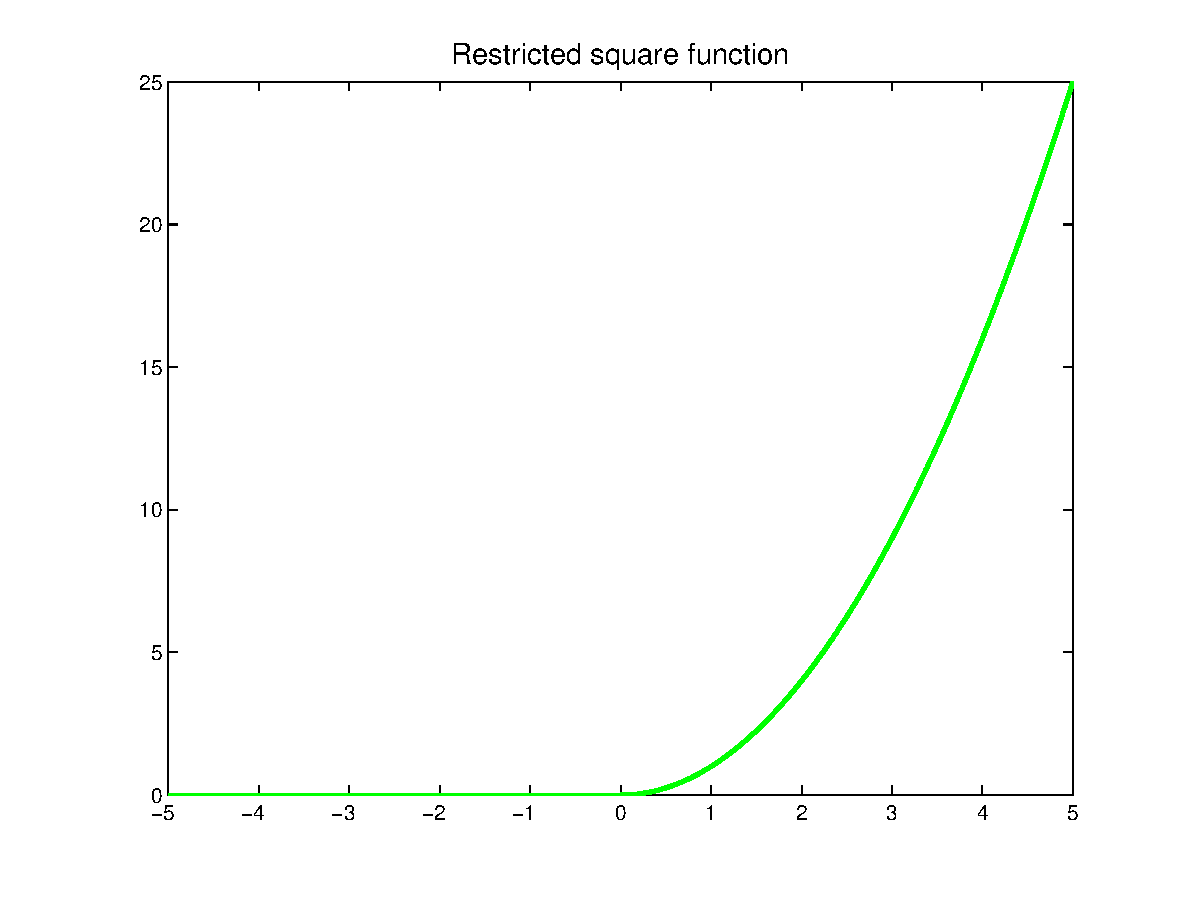
\includegraphics[scale=0.5]{./images/Course4_restrictedsquare.eps}
\caption{Restricted square function}
\label{restricted}
\end{center}
\end{figure}

\begin{example}
\begin{leftbar}
The function $\big[ \log(x+y)_+\big]^2$ is convex. Indeed, the restricted square \textcolor{red}{(is convex and increasing???)} and $-\log$ are convex functions. Therefore, their composition is convex. Since $x+y$ is a linear transformation, it preserves convexity and the whole function is convex. 
\end{leftbar}
\end{example}
\vspace{0.5cm}
\begin{property}\label{product}
If f and g are both convex, positive and increasing then their product is convex.
\end{property}
\begin{proof}
Again, one proves it in the simple differentiable, one-dimensional case. 
One has:
$$(fg)'' = \big[ f'g + fg'\big]' = f''g + 2f'g'+fg''$$
The result follows immediately since by assumptions one has $f,g,f',g',f'',g'' \geq 0$.  
\end{proof}
\textbf{Remark}: The previous proof tends to indicate variants of Property \ref{product}. One can see that if $f$ and $g$ are both concave, decreasing and negative then the proposition still holds.  

\subsection{Advantage of convex problems}
\begin{property}
Let's recall that $ \min_{x \in X} f(x)$ is convex if $f$ is convex, $X$ is convex and we are looking for a minima. We study the properties of a convex problem:
\vspace{0.5cm}
\begin{center}
 \begin{tabular}{p{7cm}|p{7cm}} 
    MODEL & METHODS \\
    \hline
	  & \\
  - Local minima are also global & - Methods which only work on convex problems: first order, second order...  \\
   - The set of optimal solutions is convex & \\
	& \\
    - Using duality we can get guarantees & \\
 \end{tabular}
 \end{center}

 \end{property}
 \subsection{Variants of convex functions}
 It's a difficult thing to know if a problem has a unique solution. There is one class of problems with only one solution: minimization of strictly convex functions.
 \vspace{0.5cm}
 \begin{definition}
 Strict convexity: $f$ is strictly convex if and only if 
 \begin{itemize}
 \item The domain is convex
 \item $f(\lambda x + (1-\lambda)y)<\lambda f(x) + (1-\lambda) f(y)$ $\forall x,y \in \textnormal{Dom}$ , $\forall \lambda \in ]0,1[$
 \end{itemize}
 \end{definition}
\vspace{0.5cm}
 \begin{example}
 \begin{leftbar}
 On the following graph, we can observe that the function is strictly convex.
 \begin{center}
 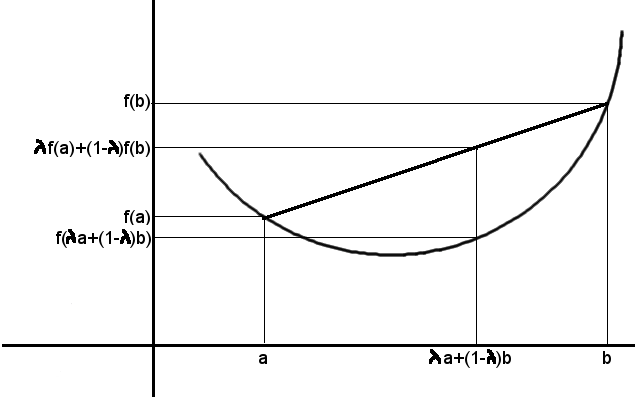
\includegraphics[scale=0.4]{./images/Course4_courbe}
 \end{center}
 \end{leftbar}
 \end{example}
\vspace{0.5cm}
\begin{example}
\begin{leftbar}
The absolute function is not strictly convex. In fact, when we have a flat part in the graph, it can not be strictly convex.
\begin{center}
  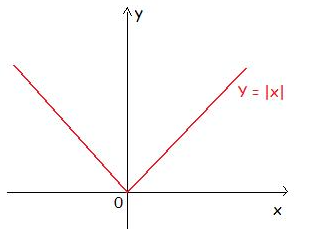
\includegraphics[scale=0.5]{./images/Course4_absolue}
\end{center}
\end{leftbar}
\end{example}
\vspace{0.5cm}
\begin{example}
\begin{leftbar}
The function $x \mapsto ||x||_{2} = \sqrt{\sum_{i} x_{i}^{2}}$ is convex but not strictly convex.
\end{leftbar}
\end{example}
\vspace{0.5cm}
\begin{property}
If we have $\min f(x)_{x \in X}$ with $f$ strictly convex and $X$ a convex set then the problem admit at most one solution.
\end{property} 
\vspace{0.5cm}
\begin{property}
If $ f \in C^{2}$ and $\nabla^{2} f(x) > 0 $ then $f$ is strictly convex. ($\lambda_{i} > 0 $ $\forall i$)
\end{property}
\vspace{0.5cm}
\begin{property}
If $f$ is convex, then $ f + ||x||^{2}_{2}$ is strictly convex.
\end{property}
\begin{proof}
Assume $f \in C_2$ 
\\then $$\nabla^{2}(f + ||x||^{2}) = \nabla^{2} f  + \nabla^{2}||x||^{2}_{2} = \nabla^{2} f + 2I
$$
where $||x||_{2}^{2} = \sum_{i} x_{i}^{2}$ and $\lambda_{i} \geq 0$.
\end{proof}
\vspace{0.5cm}
\begin{property}
$$(1) \ \lambda \text{ is an eigenvalue of } M$$
$$\Leftrightarrow$$
$$(2) \ \lambda + \Delta \text{ is an eigenvalue of } M + \Delta I$$
\\for any $\Delta \in \mathbb{R}$ and $M \in \mathbb{R}^{n \times n}$ symmetric.
\end{property}
\begin{proof}
$$ (1) \ \exists v \: \ M v = \lambda v $$
$$(2) \ \exists v \: \ (M + \Delta I) v = ( \lambda + \Delta)v$$
\end{proof}
\textbf{Remark}: We can have the same propositions and the same proof while adding $\mu > 0$ anywhere: $ f + \mu ||x||^{2}$. It is a regularization to make it strictly convex.\\
\textbf{Remark}: There are functions that have no derivative and are strictly convex.